% !TEX root=../main.tex

\chapter{ICARUS-T600 detector operations and event reconstruction}
\label{chap:event_reconstruction}

The ICARUS detector, described in \autoref{sec:ICARUS_T600} is a complex system, and a precise operation is required to make the most out of all its subcomponents. Each part of the online operation is essential and preliminary to the offline operations, consisting of the wireplane signal processing, the reconstruction of all the signals coming from the different subsystems and their combination to obtain a final physics result. 

\section{Data acquisition} \label{sec:DAQ}

The data that comes out of the detector is, much like many other experiments, organised in events. The definition of an event is unique to each experiment, as different experiments collecting different data might prefer one classification  type over another. In the case of LArTPC, an event is defined as the collection of the readout signal from all the wires, each with information on the wire position and orientation, and the raw waveform coming from all the other subdetectors modules --- CRT and PMT --- collected in a time window defined by the properties of each detector starting from a defined $t_0$. Being PMTs a fast technology, the time window of the collected waveforms is smaller than, for example, that of the TPC. The start time $t_0$ is usually defined by means of a triggering system. 

\paragraph{ICARUS trigger} The ICARUS trigger employs the coincidence between the signal from the beams (BNB and NuMI) spill gates with the scintillation light to provide a global signal that activates  the acquisition windows for the TPC and PMT subsystems. For TPC, the acquisition window is driven by the time it takes for drift electrons to cross half of each T300 module: with a nominal electric drift field of \SI{500}{\volt\per\cm}, and a half-width of $\sim\SI{1.5}{\m}$, the drift time is chosen to be $\SI{1.6}{\ms}$. The acquisition window for PMTs is driven by the mean lifetime of LAr excited states. De-excitation of LAr produces scintillation light in two components, one fast $\tau\simeq \SI{6}{\ns}$ and one slow $\tau\simeq\SI{1.6}{\us}$. To collect the full scintillation light, the time window has to be thus greater than \SI{1.6}{\us}. Additionally, in the case of a second light trigger in the \SI{10}{\us} immediate subsequent window --- this could be the case for a cosmic-induced muon crossing the detector during the drifting of the electrons ---, the readout is extended by \SI{7}{\us}. Finally, a \SI{7}{\us} buffer before the global trigger is also kept, adding up to a total of \SI{26}{\us} of PMT acquisition window.  

The ICARUS trigger architecture allows for multiple configurations, i.e. the acquisition of different types of events \cite{ICARUS:2025kai}, with and without beam (on- and off-beam), and requiring or not requiring the PMT light signal (majority or minimum bias). The main ICARUS trigger physics configuration (on-beam majority) is based on the multiplicity of PMT signals in coincidence with the beam ``open'' spill gate. Off-beam cosmic ray events are collected with similar ``off-beam majority'', requiring the coincidence between the light signal and off-beam gates, generated \SI{33}{\ms} after on-beam gates. Minimum bias (both for on- and off-beam configurations) triggers are generated in the presence of the corresponding gate, regardless of the presence of scintillation light.

\paragraph{Collection of the triggered events. } Once a global trigger is present, the data acquisition system (DAQ), which communicates via TCP/IP protocol with the trigger system, activates the readout of the whole detector, with \SI{1.6}{\ms} and \SI{26}{\us} for the TPC and PMTs, respectively. ICARUS DAQ is based on the \emph{artdaq} data acquisition software development kit developed at Fermilab \cite{Biery:2013cda}. The \emph{artdaq} SDK provides  customisable applications for reading data fragments from detector elements, which are identified as \emph{BoardReader} objects in the \emph{artdaq} language, and configurable applications for performing event-building (i.e. merging together the collected data fragments from each \emph{BordReader}, performed by objects inherited from \emph{EventBuilder} instances), data-logging and data-dispatch to downstream online data quality monitoring processes. 

Customised \emph{BoardReaders} acquire data fragments from all ICARUS subdetectors, TPC, PMT and CRT readout electronics, and from trigger and White Rabbit: this latter subsystem, not described in \autoref{sec:ICARUS_T600}, is a CERN-developed technology that provides global timing across all subdetectors and serves also as a double check against trigger global timing. Event counters and timestamps are assigned accordingly to each data fragment, which are then queued for data transfer to a configurable number of \emph{EventBuilder} instances. When an event is triggered, the corresponding trigger \emph{BoardReader} instance sends the trigger data fragment to the \emph{EventBuilder}. This triggers a request for data from all other configured \emph{BoardReader}s in the DAQ system. \autoref{fig:DAQ} shows a simplified illustration of the DAQ working principle. 

\begin{figure}
    \centering
    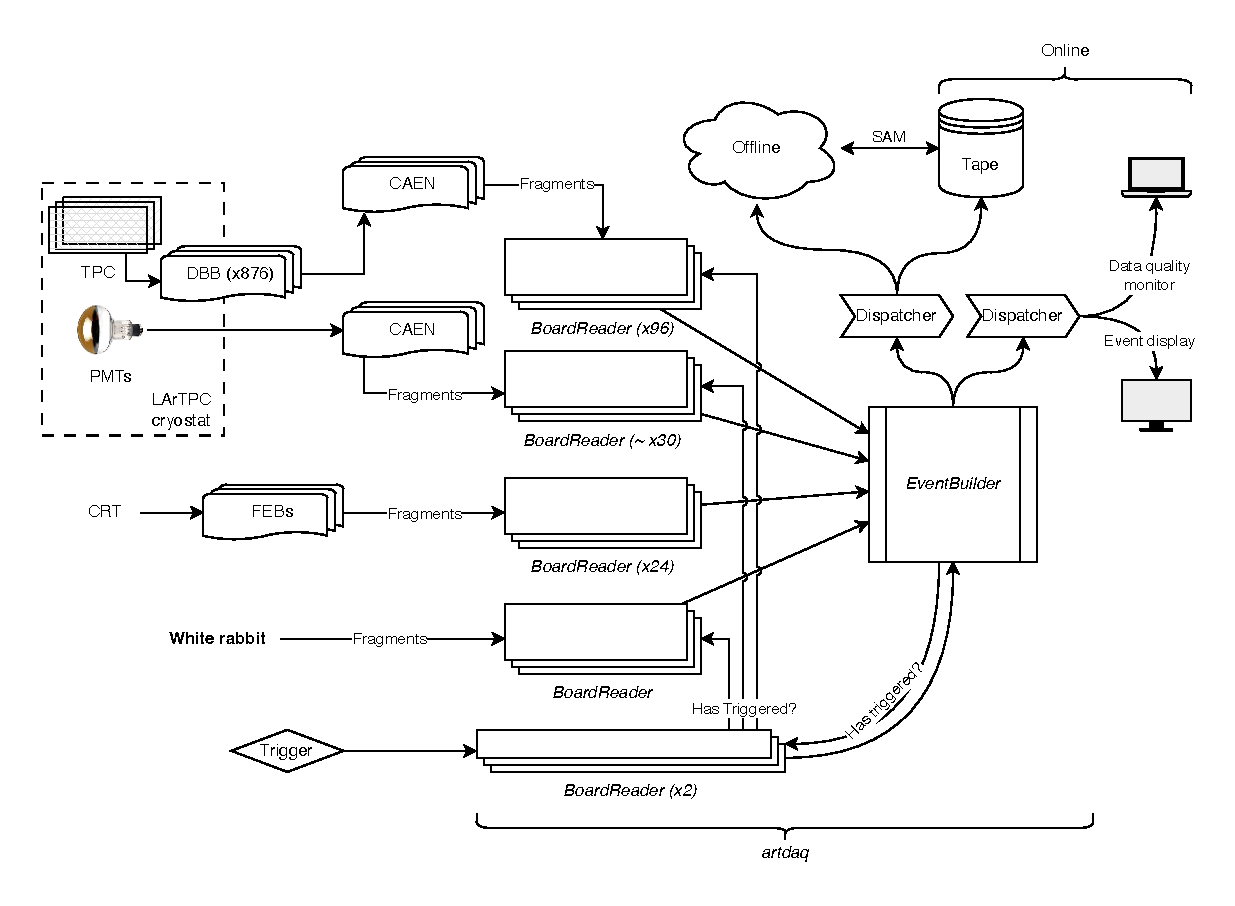
\includegraphics[width=\linewidth]{thesis/6_figures/detector/DAQ_simplified.pdf}
    \caption[ICARUS DAQ illustration]{Simplified illustration of the ICARUS DAQ system. Further information is found in \autoref{sec:DAQ}. The number of parallel \emph{EventBuilder} instances could be defined $\geq1$, to allow for faster processing.}
    \label{fig:DAQ}
\end{figure}

The data collected by the ICARUS DAQ system is written in different file streams depending on which beam it is detecting and which trigger configuration is active, whether on- or off-beam, minimum bias or majority. 

Downstream of the DAQ interface, events are written using the \emph{art} event-processing framework \cite{greenArtFramework2012} also developed at Fermilab, on which the \emph{artdaq} SDK is built. This allows flawless interoperability between the DAQ interface and the offline analysis, without the need to convert the events saved from the DAQ interface into a format compatible with the high-level offline analysis. After a long testing and commissioning phase, the DAQ system was reported to be able to stably handle high data rates up to \SI{5}{\hertz}. This is, however, well in excess of what the detector is supposed to be handling, given the BNB and NuMI data rates when using a majority-based trigger configuration, based on light scintillation, delivering about \SI{1}{\hertz} of data throughput.  

In order to handle the large volumes of data stored on tape, the Fermilab-based SAM (serial access to metadata) system is exploited. This system associates a set of metadata information with each data file using Python scripts. This metadata is useful in offline analysis to create large datasets of files, identifying whether the files contain raw or processed data, run configuration, run number and so on.

\section{ICARUS data processing}

The output data files contain the aggregated data coming from all the \emph{BoardReader} instances in an event. For the TPC, the data correspond to the digitised waveforms from each TPC readout channel, representing the charge induced by the motion of ionisation electrons drifted by the electric field inside the detector. Similarly, the data from the PMTs correspond to the digitised waveforms of the readout of every PMT inside the detector, corresponding of the scintillation light deposited in each PMT. For the CRT system the DAQ process is slightly different \cite{ICARUS:2025rdw,Poppi:2023zmp,Poppi:2022vhg}. The ICARUS CRTs operate in self-trigger mode \cite{arteroponsStudyReconstructionNuMuCC, ICARUS:2025rdw}, whenever a CRT SiPM exceeds the threshold, the data from all 32 SiPM channels for each FEB is stored in internal buffers, holding up to \qtyrange{40}{80}{\ms} depending on which CRT sub-part is considered. The data from the top, bottom and side CRTs is aggregated within \SI{10}{\us} data fragments in the \emph{BoardReader}s instances; once the global trigger is activated, \SI{+-25}{\ms} of CRT data fragments are sent from the \emph{BoardReader} to the \emph{EventBuilder} instance. 

The output of all ICARUS sub-detectors is common across LArTPC detectors, which might have different TPC geometry and light collection configurations but share the same underlying technology. The \emph{art}-based \emph{LArSoft} framework \cite{Church:2013hea,Snider:2017wjd,Pordes:2017BL} is the common software development kit providing software infrastructure and algorithms for simulation of Monte Carlo data, processing of both simulated and real data, and event reconstruction. 

When an event is saved from DAQ to data files and stored to tape, it is then available to be processed. The ICARUS data processing chain is split, like for many other LArTPC detectors, into two \emph{stages}, usually named \emph{Stage0} or \emph{reco1} and \emph{Stage1} or \emph{reco2}. Processing the raw collected data is a mandatory step in order for it to be properly analysed. 

In the \emph{Stage0/reco1} step, all data  from the three sub-detectors is processed to produce a ``simpler'' description of the raw signal. This means to decode the raw signal and translate it into objects in the \emph{LArSoft} format for offline reconstruction. It also performs signal processing of the waveforms to identify physical signals, \emph{Hits}, that can then be used as input to the higher-level event reconstruction tools implemented in the \emph{Stage1/reco2} steps. 

% path: [
%       "pmtfixedthr",
%       "pmtlvdsgates",
%       "pmttriggerwindows",
%       "triggersimgates",
%       "emuTrigger",
%       "pmtbaselines",
%       "ophit",
%       "mcophit",
%       "opflashCryoE",
%       "opflashCryoW",
%       "MCDecodeTPCROI",
%       "decon1droi",
%       "roifinder1d",
%       "gaushit1dTPCEW",
%       "gaushit1dTPCEE",
%       "gaushit1dTPCWW",
%       "gaushit1dTPCWE",
%       "purityana0",
%       "purityana1",
%       "simChannelROI",
%       "crthit",
%       "crttrack",
%       "crtpmt"
%    ]


%  reco: [
%       "cluster3DCryoE",
%       "pandoraGausCryoE",
%       "pandoraTrackGausCryoE",
%       "pandoraKalmanTrackGausCryoE",
%       "SBNShowerGausCryoE",
%       "cluster3DCryoW",
%       "pandoraGausCryoW",
%       "pandoraTrackGausCryoW",
%       "pandoraKalmanTrackGausCryoW",
%       "SBNShowerGausCryoW",
%       "fmatchCryoE",
%       "fmatchCryoW",
%       "fmatchopCryoE",
%       "fmatchopCryoW",
%       "tpcpmtbarycentermatchCryoE",
%       "tpcpmtbarycentermatchCryoW",
%       "caloskimCalorimetryCryoE",
%       "caloskimCalorimetryCryoW",
%       "mcassociationsGausCryoE",
%       "mcassociationsGausCryoW"
%    ]


\section{Light reconstruction}

\section{Cosmic ray ragger reconstruction}

\section{TPC event reconstruction}

\subsection{Wireplanes signal processing}

\subsection{Sequential approach: Pandora}

\subsection{Machine Learning approach: SPINE}

